%# -*- coding:utf-8 -*-
\subsection[心脏分割]{基于测地活动轮廓的心脏近似区域分割}

\begin{frame}
\begin{itemize}
\item \textbf{血管介入仿真中心脏表面模型的作用}
\begin{itemize}
\item 增强虚拟解剖环境的视觉效果
\item 为辨认冠状动脉模型的不同分支提供空间参照物
\end{itemize}
\pause \item \textbf{血管介入仿真中心脏表面模型的获取}
\begin{itemize}
\item 几何形状近似的椭球或者不规则的几何体
\item 未考虑心脏表面模型
\item 医学影像处理方法
\end{itemize}
\pause \item \textbf{心脏近似区域的分割与可视化}
\begin{itemize}
\item 是医学影像领域中的一项极具挑战性的工作
\item 形态特征:不规则的空间形体,可近似看作椭球
\item 分割时的主要困难:搏动致心脏边缘模糊不清,且帧间变化大
\begin{itemize}
\item 只分割心脏的近似区域,得到近似模型,满足仿真需要
\end{itemize}
\end{itemize}
\end{itemize}
\end{frame}

\begin{frame}
\begin{itemize}
  \item \textbf{心脏区域分割流程}:
\end{itemize}
\begin{figure}[t]
\centering
%# -*- coding:utf-8 -*-
\begin{tikzpicture}[scale=.37]

\draw [black,thick,rounded corners] (-3,0) rectangle (3,2);            % binary threshold
\draw [black,thick,rounded corners] (-3,3) rectangle (3,5);  % CURVES

\draw [black,thick,rounded corners] (-8,7) rectangle (-2,9);   % initial contours

\draw [black,thick,rounded corners] (2,7) rectangle (8,9);     % feature images

\draw [black,thick,rounded corners] (-3,11) rectangle (3,13);  % thresholding
\draw [black,thick,rounded corners] (-3,14) rectangle (3,16);  % curvature anisotropic diffusion
\draw [black,thick,rounded corners] (-3,17) rectangle (3,19);  % raw input

\node [above right] at (-2.25,0.25) {\scriptsize \fs \bf 二值阈值滤波};
\node [above right] at (-2.25,3.25) {\scriptsize \fs \bf 测地活动轮廓};

\node [above right] at (-7.65,7.35) {\scriptsize \fs \bf 初始水平集演进};

\node [above right] at (2.82,7.35) {\scriptsize \fs \bf 特征图像计算};

\node [above right] at (-2.3,11.35) {\scriptsize \fs \bf 二值阈值滤波};
\node [above right] at (-2.9,14.35) {\scriptsize \fs \bf 曲率各向异性扩散};
\node [above right] at (-1.95,17.35) {\scriptsize \fs \bf ROI体数据};

\draw [<-,thick] (0,2) -- (0,3);

\draw [<-,thick] (0,5) -- (0,6);
\draw [thick] (-5,6) -- (5,6);
\draw [thick] (-5,6) -- (-5,7);
\draw [thick] (5,6) -- (5,7);

\draw [<-,thick] (-5,9) -- (-5,10);
\draw [<-,thick] (5,9) -- (5,10);
\draw [thick] (-5,10) -- (5,10);
\draw [thick] (0,10) -- (0,11);

\draw [<-,thick] (0,13) -- (0,14);
\draw [<-,thick] (0,16) -- (0,17);

\end{tikzpicture} 
% 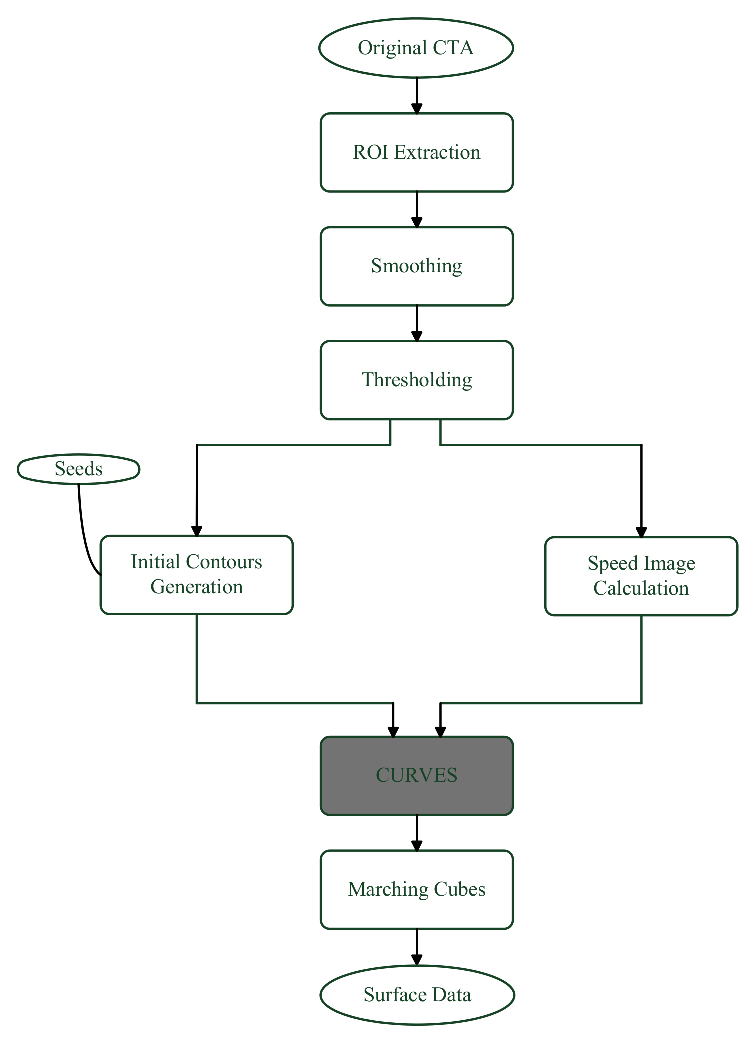
\includegraphics[height=2.0in]{figures/heart/DataFlow.eps}
% \caption[心脏区域分割流程]{心脏区域分割流程。}
% \label{fig:heart_data_flow}
\end{figure}
\end{frame}

% \begin{frame}
% \begin{itemize}
  % \item \textbf{心脏区域前面观}:
% \end{itemize}
% \begin{figure}[t]
% \centering
% 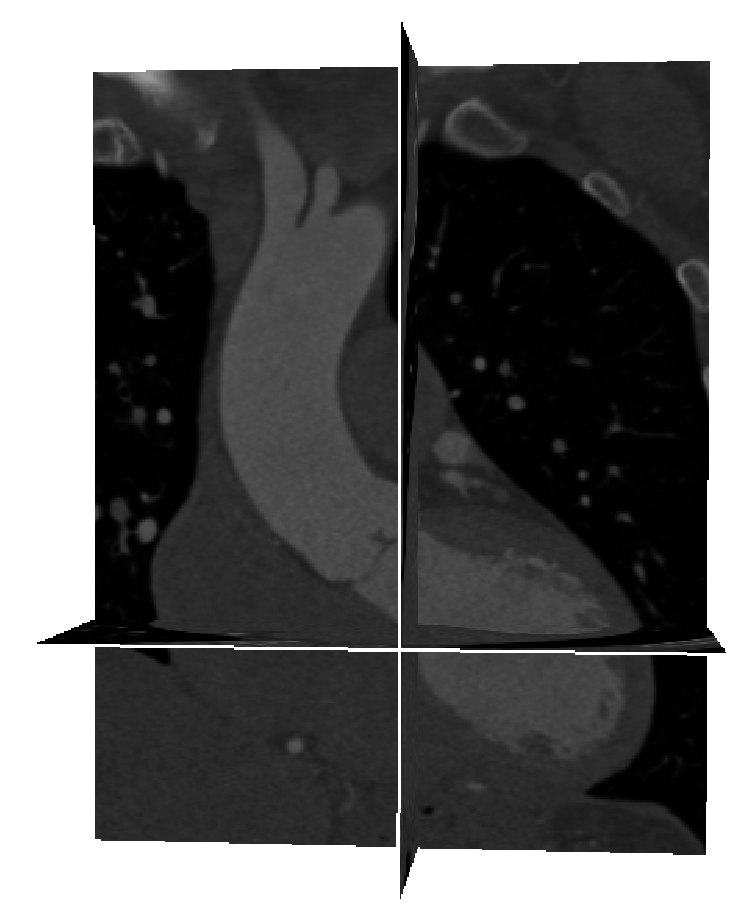
\includegraphics[height=1.5in]{../../Figures/gac/heart/original.eps}
% \end{figure}
% \end{frame}

\begin{frame}
\begin{itemize}
  \item \textbf{二值阈值后心脏区域前面观}:
  \begin{itemize}
    \onslide<1-2> \item 阈值滤波($\text{TH}_{\text{lower}} = 0$,$\text{TH}_{\text{upper}} = 200$)
    \onslide<2> \item 注意其中的心脏组织以及大部分血管等都已被除去
  \end{itemize}
\end{itemize}
% \begin{figure}[t]
% \centering
% 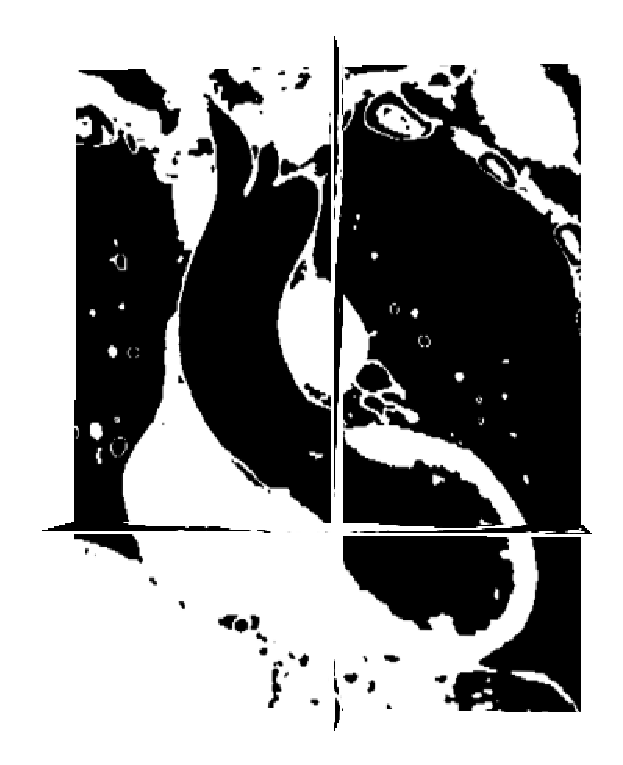
\includegraphics[height=1.5in]{../../Figures/gac/heart/binary_threshold.eps}
% \caption[二值阈值后心脏区域前面观]{二值阈值后心脏区域前面观($\text{TH}_{\text{lower}} = 0$,$\text{TH}_{\text{upper}} = 200$)。注意其中的心包,以及大部分血管等都已被除去。}%
% \label{fig:heart_binary_threshold_experiments}
% \end{figure}
\begin{columns}[b,onlytextwidth]
\begin{column}{.5\textwidth}
\onslide<1-2> \begin{figure}
\centering
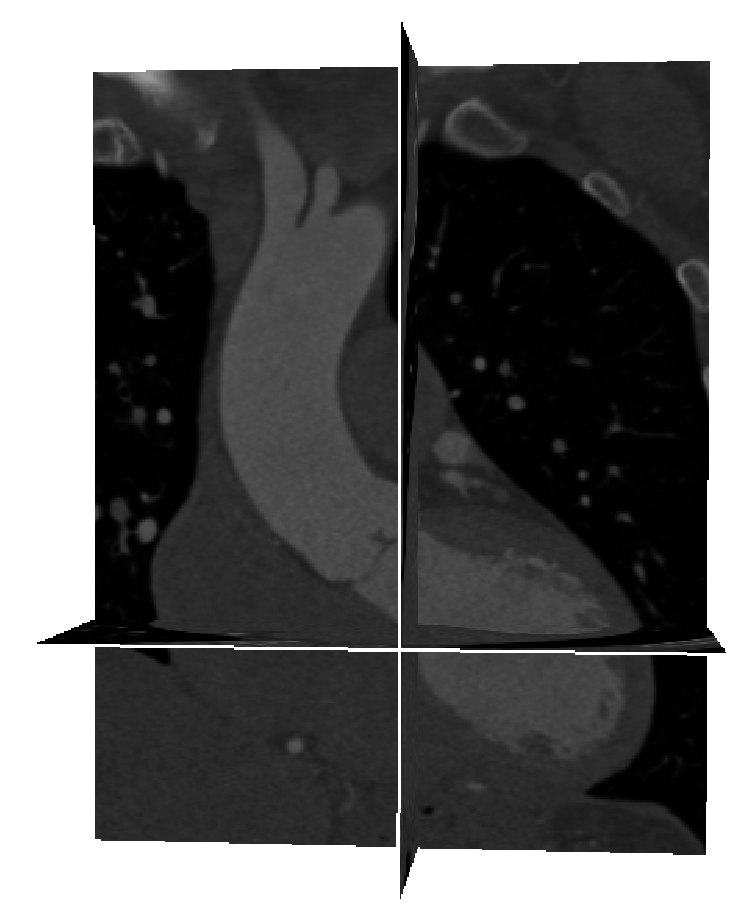
\includegraphics[height=1.5in]{../../Figures/gac/heart/original.eps}
\end{figure}
\end{column}
\begin{column}{.5\textwidth}
\onslide<2> \begin{figure}
\centering
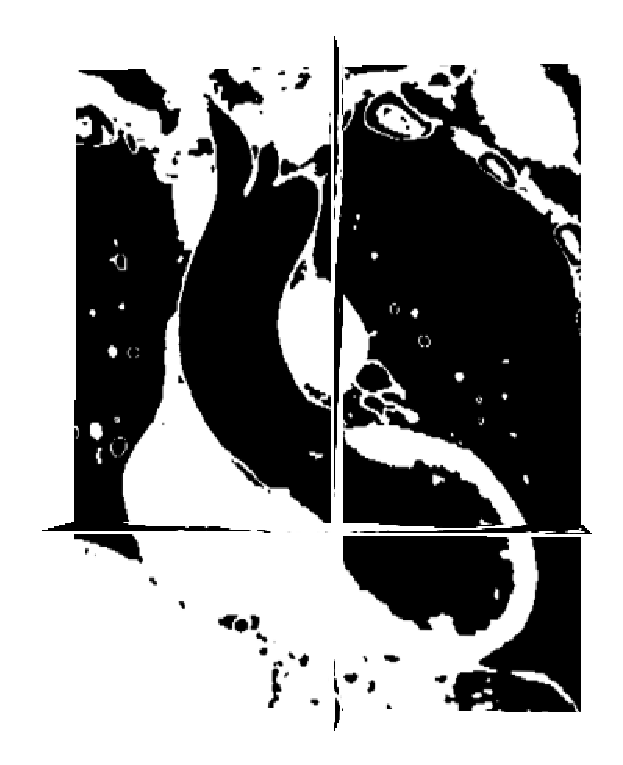
\includegraphics[height=1.5in]{../../Figures/gac/heart/binary_threshold.eps}
\end{figure}
\end{column}
\end{columns}
\end{frame}

\begin{frame}
\begin{itemize}
  \item \textbf{心脏表面模型前面观}:
  % \begin{itemize}
    % \item $\text{TH}_{\text{lower}} = 0$,$\text{TH}_{\text{upper}} = 200$
    % \item 注意其中的心包,以及大部分血管等都已被除去
  % \end{itemize}
\end{itemize}
\begin{figure}[t]
\centering
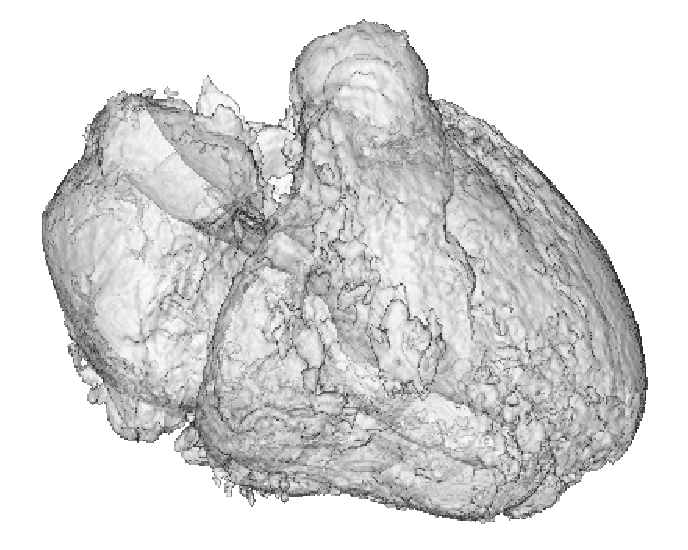
\includegraphics[height=1.5in]{../../Figures/gac/heart/heart.eps}
% \caption[二值阈值后心脏区域前面观]{二值阈值后心脏区域前面观($\text{TH}_{\text{lower}} = 0$,$\text{TH}_{\text{upper}} = 200$)。注意其中的心包,以及大部分血管等都已被除去。}%
% \label{fig:heart_binary_threshold_experiments}
\end{figure}
\end{frame}

\begin{frame}
\begin{itemize}
  \item \textbf{叠加冠状动脉(红色)的心脏模型前面观}:
  % \begin{itemize}
    % \item $\text{TH}_{\text{lower}} = 0$,$\text{TH}_{\text{upper}} = 200$
    % \item 注意其中的心包,以及大部分血管等都已被除去
  % \end{itemize}
\end{itemize}
\begin{figure}[t]
\centering
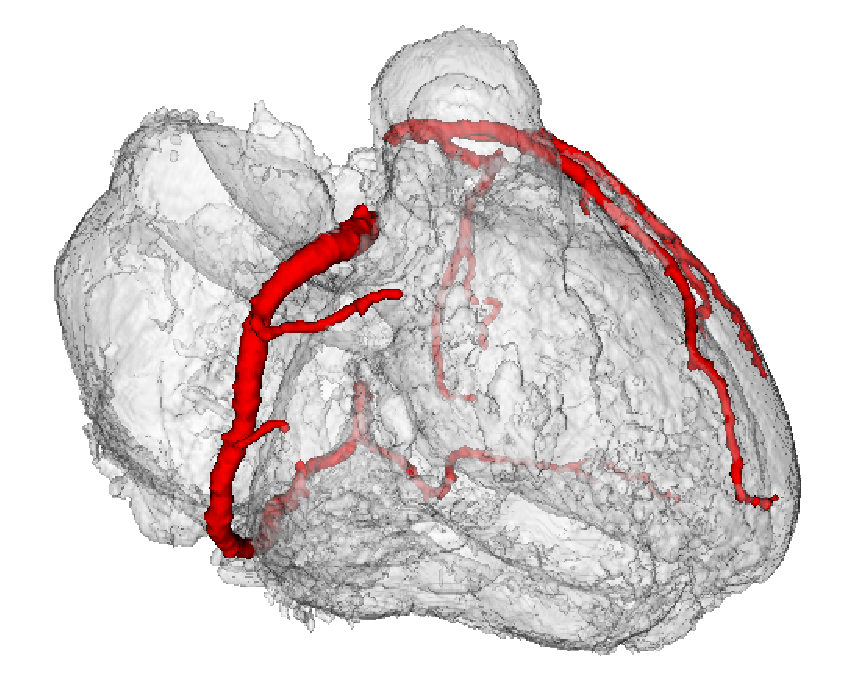
\includegraphics[height=1.5in]{../../Figures/gac/heart/heart_with_ca.eps}
% \caption[二值阈值后心脏区域前面观]{二值阈值后心脏区域前面观($\text{TH}_{\text{lower}} = 0$,$\text{TH}_{\text{upper}} = 200$)。注意其中的心包,以及大部分血管等都已被除去。}%
% \label{fig:heart_binary_threshold_experiments}
\end{figure}
\end{frame} 

% \begin{frame}

% \end{frame} 
 